\chapter{評価}
\begin{large}
\begin{quote}
本章では,T-Ringシステムの評価を行う.
\end{quote}
\end{large}
\clearpage

\section{評価方針}
本研究では,センサデータを多次元データとして扱う際に,時間を他の属性と同様に扱っているSynapseと,センサデータの時間的特殊性を考慮したT-Ringの取得時間の比較を行う.
Synapseの手法では,保存,取得の際に,データごとにFinger Tableによる保存ピアの探索を行わなければならない.よって,本評価では,ネットワークに参加するピア数を固定し,データの保存,取得に共通する,保存ピア探索の計算コストを計測する.次に,保存時,取得時に分けて探索に要する時間の計測を行う.
%本研究に評価では,まず,ネットワークに参加する保存ピアの数を固定し,単位時間における取得のクエリ数を段階的に増やし,全ての情報の取得が終了するまでにどれだけの時間がかかるかを評価する.次に,ネットワーク内の保存ピア数により,一回の保存ピア探索のホップ数が変化するので,単位時間における取得のクエリ数を固定し,ネットワークに参加する保存ピアの数を変化させる.
%取得の対象データは,評価結果に影響を与えないが,センサデータであることを考慮し,サイズは2バイトとする.

\section{評価環境}
本研究は,評価環境として,慶応義塾大学湘南藤沢キャンパス内の特別教室内に設置されている124台のiMacの内,任意の複数マシンを用いて行う.詳細なスペックなどについては以下の表\ref{tab:information}で示す.

\begin{table}[htb]
  \centering
  \caption{実験環境}
  \begin{tabular}{|c||c|} \hline
  	ホスト名	 & zmac000-159 \\ \hline
	本体 & iMac 21.5 インチ \\ \hline
	CPU	& 3.06 GHz Intel Core 2 Duo \\ \hline
	メモリ & 4 GB (2 GB X 2) \\ \hline
	ハードディスク	& 499.76 GB \\ \hline
	OS & Mac OS X 10.6.5 \\ \hline
  \end{tabular}
  \label{tab:information}
\end{table}
\subsection{実験環境内におけるネットワークレイテンシ}
本研究では,データの保存や探索に要する時間を計測するため,各保存ピア間の通信におけるレイテンシが重要になる.そこで,本実験環境におけるマシン間のレイテンシが実験にどの程度の影響を与えるのかを調査するため,事前実験として,各リージョン間のRTTを計測した.各リージョンがどこに存在するかは,図\ref{fig:region}において示す.それぞれICMPにおけるEcho Messageを送信し,リプライが返されるまでの時間の計測を100回行い,その平均値,最小値,最大値,標準偏差を表\ref{tab:ping_regionA},\ref{tab:ping_regionB},\ref{tab:ping_regionC},\ref{tab:ping_regionD}で示す.本実験において,実験環境下ではRTTが0.400ms以下であるという知見が得られた.本システムが用いられる実環境におけるRTTは0.400msより十分に大きいため,本評価では,実験環境内におけるネットワークレイテンシを無視する.


 \begin{figure}[htbp]
 %\begin{minipage}{0.5\hsize}
  \begin{center}
   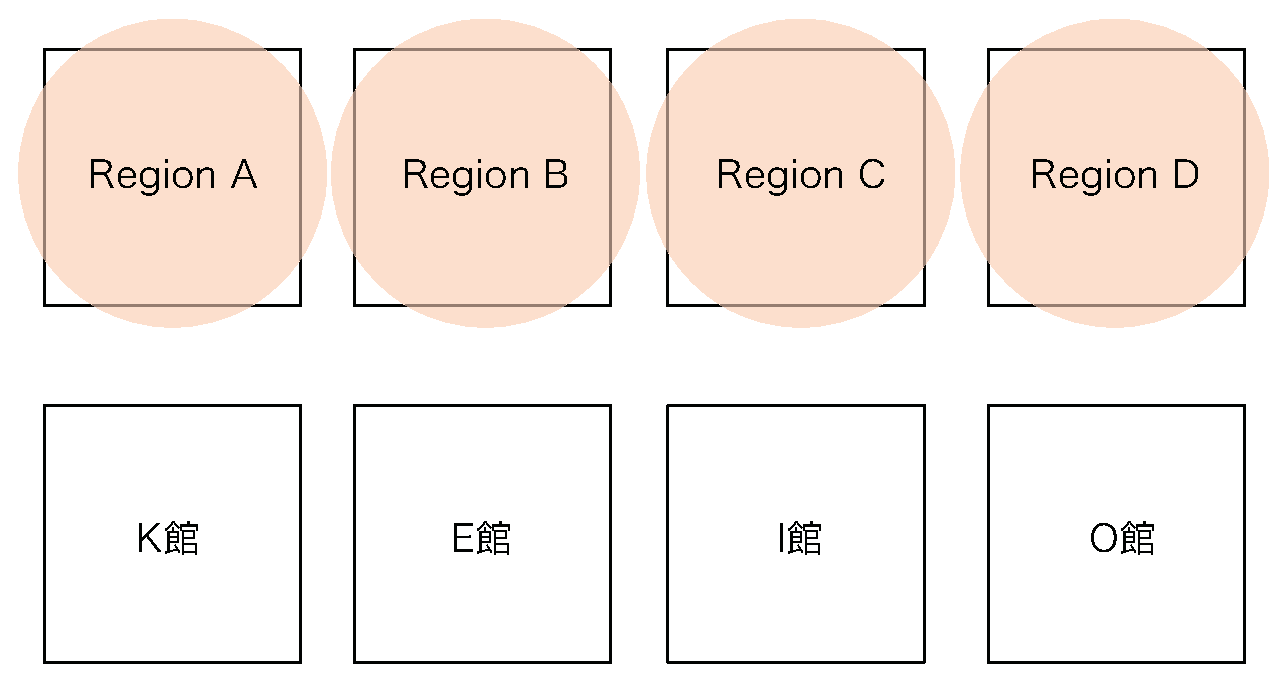
\includegraphics[width=140mm]{./images/region.eps}
  \end{center}
  \caption{リージョンの関係性}
  \label{fig:region}
 %\end{minipage}
\end{figure}

\begin{table}[htb]
  \centering
  \caption{リージョンAからのRTT}
  \begin{tabular}{|c||c|c|c|c|} \hline
    \backslashbox{}{} & 平均値 & 最小値 & 最大値 & 標準偏差 \\ \hline \hline
    リージョンA & 0.234 ms & 0.193 ms & 0.271 ms & 0.022 \\ \hline
    リージョンB & 0.324 ms & 0.287 ms & 0.349 ms & 0.015 \\ \hline
    リージョンC & 0.321 ms & 0.285 ms & 0.347 ms & 0.016 \\ \hline
    リージョンD & 0.315 ms & 0.277 ms & 0.339 ms & 0.016 \\ \hline
  \end{tabular}
  \label{tab:ping_regionA}
\end{table}

\begin{table}[htb]
  \centering
  \caption{リージョンBからのRTT}
  \begin{tabular}{|c||c|c|c|c|} \hline
    \backslashbox{}{} & 平均値 & 最小値 & 最大値 & 標準偏差 \\ \hline \hline
    リージョンA & 0.327 ms & 0.288 ms & 0.347 ms & 0.015 \\ \hline
    リージョンB & 0.238 ms & 0.203 ms & 0.270 ms & 0.019 \\ \hline
    リージョンC & 0.319 ms & 0.274 ms & 0.349 ms & 0.018 \\ \hline
    リージョンD & 0.317 ms & 0.282 ms & 0.347 ms & 0.015 \\ \hline
  \end{tabular}
  \label{tab:ping_regionB}
\end{table}

\begin{table}[htb]
  \centering
  \caption{リージョンCからのRTT}
  \begin{tabular}{|c||c|c|c|c|} \hline
    \backslashbox{}{} & 平均値 & 最小値 & 最大値 & 標準偏差 \\ \hline \hline
    リージョンA & 0.325 ms & 0.277 ms & 0.359 ms & 0.016 \\ \hline
    リージョンB & 0.312 ms & 0.279 ms & 0.342 ms & 0.015 \\ \hline
    リージョンC & 0.252 ms & 0.192 ms & 0.379 ms & 0.022 \\ \hline
    リージョンD & 0.319 ms & 0.283 ms & 0.343 ms & 0.015 \\ \hline
  \end{tabular}
  \label{tab:ping_regionC}
\end{table}

\begin{table}[htb]
  \centering
  \caption{リージョンDからのRTT}
  \begin{tabular}{|c||c|c|c|c|} \hline
    \backslashbox{}{} & 平均値 & 最小値 & 最大値 & 標準偏差 \\ \hline \hline
    リージョンA & 0.296 ms & 0.240 ms & 0.727 ms & 0.047 \\ \hline
    リージョンB & 0.295 ms & 0.259 ms & 0.374 ms & 0.014 \\ \hline
    リージョンC & 0.252 ms & 0.192 ms & 0.379 ms & 0.022 \\ \hline
    リージョンD & 0.291 ms & 0.239 ms & 0.335 ms & 0.013 \\ \hline
  \end{tabular}
  \label{tab:ping_regionD}
\end{table}

\section{保存ピア探索の計算コスト}
データの保存,取得時に,Synapseでは対象のデータの時間毎に保存ピアの探索を行う一方で,T-Ringは対象のセンサーのchunk,SPの値により,探索の回数が変化する.そこで,1000個の連続したデータを保存,取得することを想定し,Synapse,T-Ringの両手法において,1データの平均のピア間ホップ数を計測する.またT-Ringにおいては,各データの時間の間隔を5,SPを100,chunkを10,30,50,70,90の5つとする.図\ref{fig:compare_hop}はその結果である.

 \begin{figure}[htbp]
 %\begin{minipage}{0.5\hsize}
  \begin{center}
   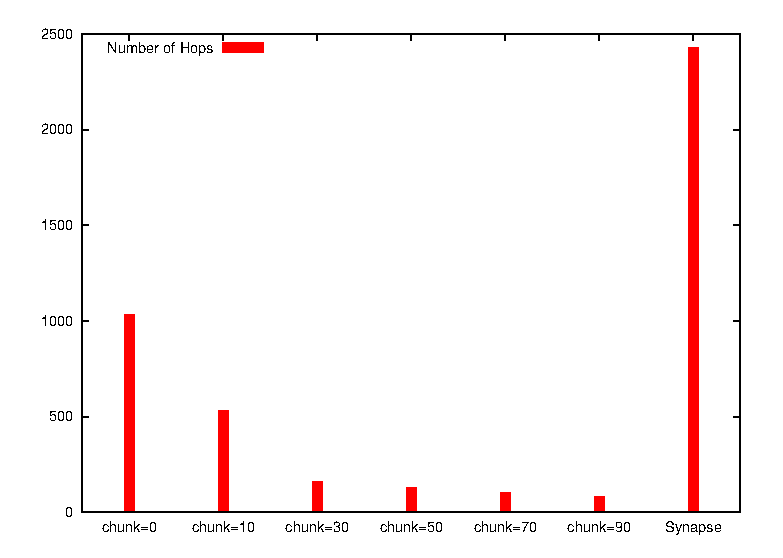
\includegraphics[width=130mm]{./images/compare_hop.eps}
  \end{center}
  \caption{ホップ数}
  \label{fig:compare_hop}
 %\end{minipage}
\end{figure}



\section{データ保存時の評価}
データの保存時にSynapseでは,データ毎に保存場所の計算を行う.その一方で,T-Ringでは,ある一定の時間が経過するまでは,保存場所の変更が発生しない.そこで,ある保存ピアに100個のデータを保存するクエリを送り,それらの保存が完了するまでの時間を計測する.本評価では,保存されるデータの設定をchunk=30,SP=100,各データの時間の間隔を5として実験を行った.また,ネットワークの環境については,ネットワークに参加している保存ピアの数(ネットワークサイズ=NS)を10,50,100の3種類,各ピア間のRTTを5,10,50,1000の4種類とした.図\ref{fig:compare_store_rtt5},\ref{fig:compare_store_rtt10},\ref{fig:compare_store_rtt50},\ref{fig:compare_store_rtt100}はRTTごとにまとめた実験結果である.

\begin{figure}[htbp]
\begin{minipage}{1\textwidth}
    \centering
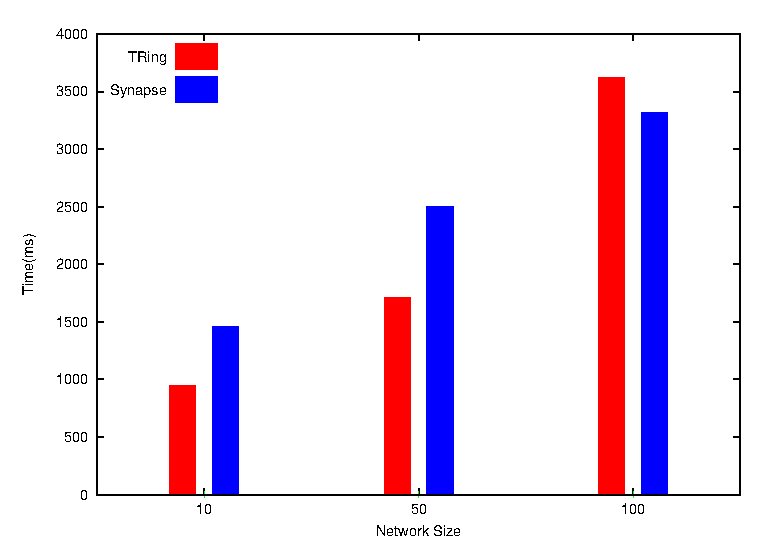
\includegraphics[width=14cm]{./images/compare_store_rtt5.eps}
\begin{center}
  \begin{tabular}{|c||c|c|c|} \hline
    \backslashbox{}{} & NS=10 & NS=50 & NS=100  \\ \hline \hline
       T-Ring & 944 ms & 1708 ms & 3625 ms  \\ \hline
       Synapse & 1458  ms & 2506 ms & 3315 ms \\ \hline
  \end{tabular}
\end{center}
\caption{保存:RTT=5}
 \label{fig:compare_store_rtt5}
 \end{minipage}
\end{figure}


\begin{figure}[htbp]
\begin{minipage}{1\textwidth}
    \centering
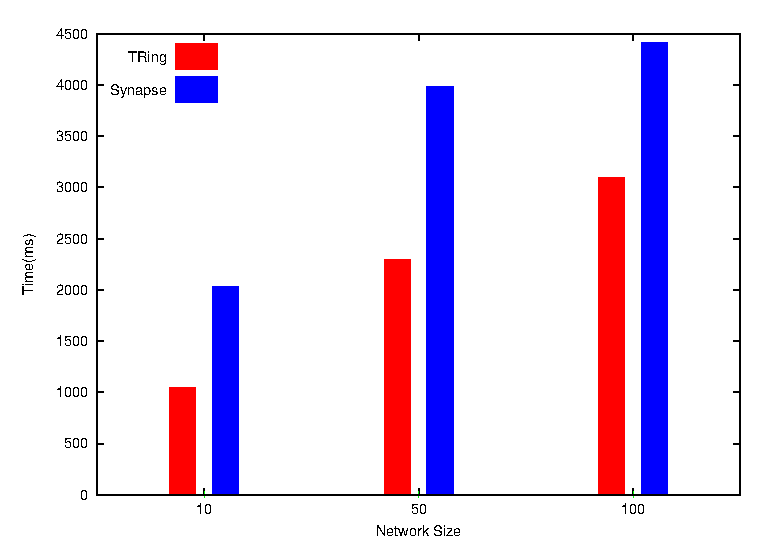
\includegraphics[width=14cm]{./images/compare_store_rtt10.eps}
 \begin{center}
 %\begin{table}[htbp]
  %\centering
  %\caption{保存:RTT=10値}
  \begin{tabular}{|c||c|c|c|} \hline
    \backslashbox{}{} & NS=10 & NS=50 & NS=100  \\ \hline \hline
       T-Ring & 1049 ms & 2300 ms & 3101 ms  \\ \hline
       Synapse & 2029  ms & 3989 ms & 4414 ms \\ \hline  \end{tabular}
  \label{tab:RTT=10}
\end{center}
\caption{保存:RTT=10}
 \label{fig:compare_store_rtt10}
 \end{minipage}
\end{figure}

\begin{figure}[htbp]
\begin{minipage}{1\textwidth}
    \centering
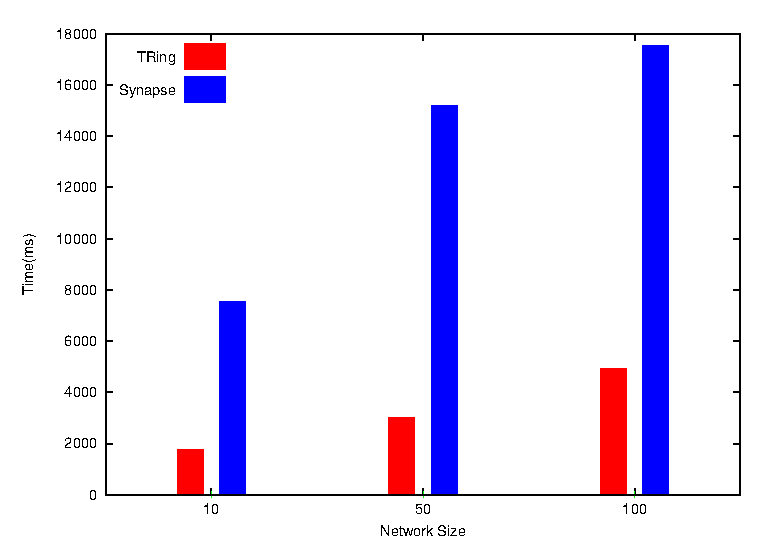
\includegraphics[width=14cm]{./images/compare_store_rtt50.eps}
\begin{center}
 %\begin{table}[htbp]
  %\centering
  %\caption{保存:RTT=50値}
  \begin{tabular}{|c||c|c|c|} \hline
    \backslashbox{}{} & NS=10 & NS=50 & NS=100  \\ \hline \hline
       T-Ring & 1049 ms & 2300 ms & 3101 ms  \\ \hline
       Synapse & 2029  ms & 3989 ms & 4414 ms \\ \hline  \end{tabular}
  \label{tab:RTT=50}
\end{center}
\caption{保存:RTT=50}
\label{fig:compare_store_rtt50}
 \end{minipage}
\end{figure}

\begin{figure}[htbp]
\begin{minipage}{1\textwidth}
    \centering
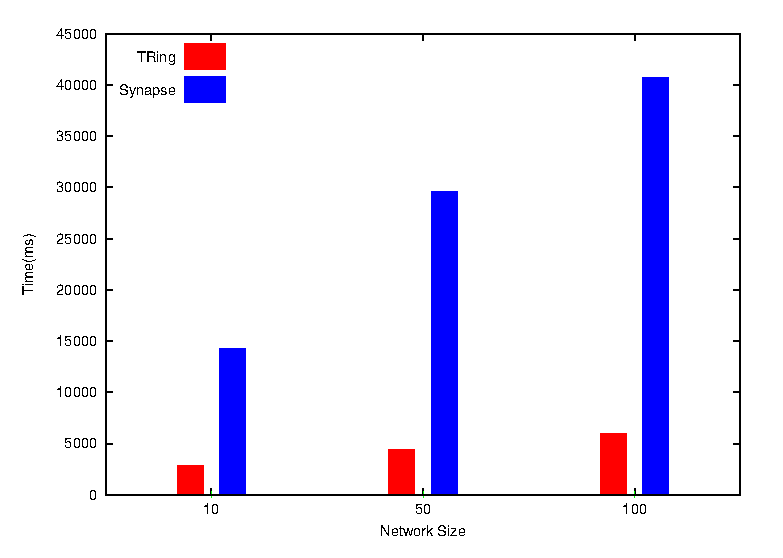
\includegraphics[width=14cm]{./images/compare_store_rtt100.eps}
%\caption{保存:RTT=100}
\begin{center}
 %\begin{table}[htbp]
  %\centering
  %\caption{保存:RTT=100値}
  \begin{tabular}{|c||c|c|c|} \hline
    \backslashbox{}{} & NS=10 & NS=50 & NS=100  \\ \hline \hline
       T-Ring & 1049 ms & 2300 ms & 3101 ms  \\ \hline
       Synapse & 2029  ms & 3989 ms & 4414 ms \\ \hline  \end{tabular}
  \label{tab:RTT=100}
\end{center}
\caption{保存:RTT=100}
\label{fig:compare_store_rtt100}
 \end{minipage}
\end{figure}




\section{データ取得時の評価}
保存時と同様に,データの取得時にSynapseでは,取得するセンサデータごとに保存場所の探索を行い,T-Ringではある一定の時間が経過するまで,取得先の変更は発生しない.そこで,ある特定の領域に対して,500単位時間のデータの取得を行うクエリを送り,データが全て返されるまでの時間を計測する.本評価では,データはすべて5単位時間ごとに保存されている環境を想定する.よって,500単位時間分のデータは,100個のデータを取得することとなる.クエリの地理的範囲は半径10の広さを持ったものとする.また,ネットワークに関しては,保存時と同様に,ネットワークに参加している保存ピアの数(ネットワークサイズ=NS)を10,50,100の3種類,各ピア間のRTTを5,10,50,1000の4種類とした.図\ref{fig:compare_retrieve_rtt5},\ref{fig:compare_retrieve_rtt10},\ref{fig:compare_retrieve_rtt50},\ref{fig:compare_retrieve_rtt100}はRTTごとにまとめた実験結果である.
%保存場所探索の計算が行われた回数,データが保存されているピアを発見に至るホップ数の総計,取得の開始から完了までの時間を計測する.また,単位時間を1分とし,クエリの送信回数を100回から10000回に漸次的に増加させる.

\begin{figure}[htbp]
\begin{minipage}{1\textwidth}
    \centering
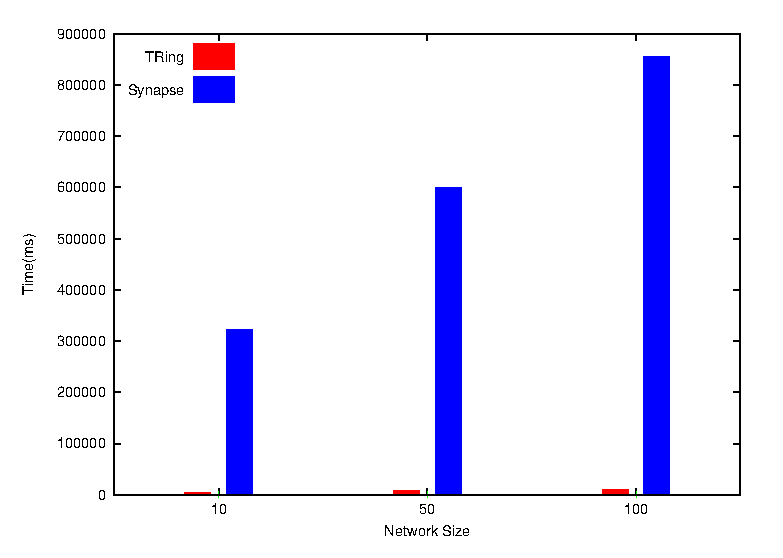
\includegraphics[width=14cm]{./images/compare_retrieve_rtt5.eps}
\begin{center}
  \begin{tabular}{|c||c|c|c|} \hline
    \backslashbox{}{} & NS=10 & NS=50 & NS=100  \\ \hline \hline
       T-Ring & 3884 ms & 8098 ms & 9823 ms  \\ \hline
       Synapse & 322615  ms & 599557 ms & 855187 ms \\ \hline
  \end{tabular}
\end{center}
\caption{取得:RTT=5}
 \label{fig:compare_retrieve_rtt5}
 \end{minipage}
\end{figure}

\begin{figure}[htbp]
\begin{minipage}{1\textwidth}
    \centering
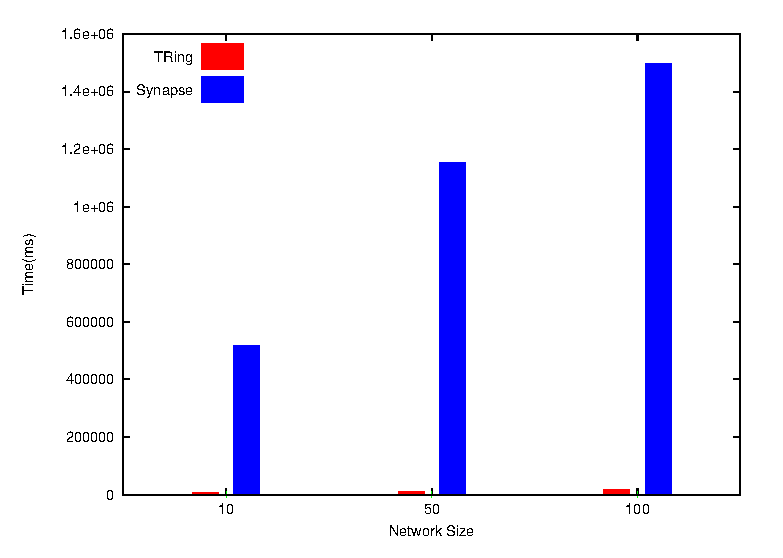
\includegraphics[width=14cm]{./images/compare_retrieve_rtt10.eps}
\begin{center}
  \begin{tabular}{|c||c|c|c|} \hline
  \backslashbox{}{} & NS=10 & NS=50 & NS=100  \\ \hline \hline
       T-Ring & 6247 ms & 12683 ms & 16249 ms  \\ \hline
       Synapse & 519541  ms & 1155219 ms & 1498550 ms \\ \hline
  \end{tabular}
\end{center}
\caption{取得:RTT=10}
 \label{fig:compare_retrieve_rtt10}
 \end{minipage}
\end{figure}

\begin{figure}[htbp]
\begin{minipage}{1\textwidth}
    \centering
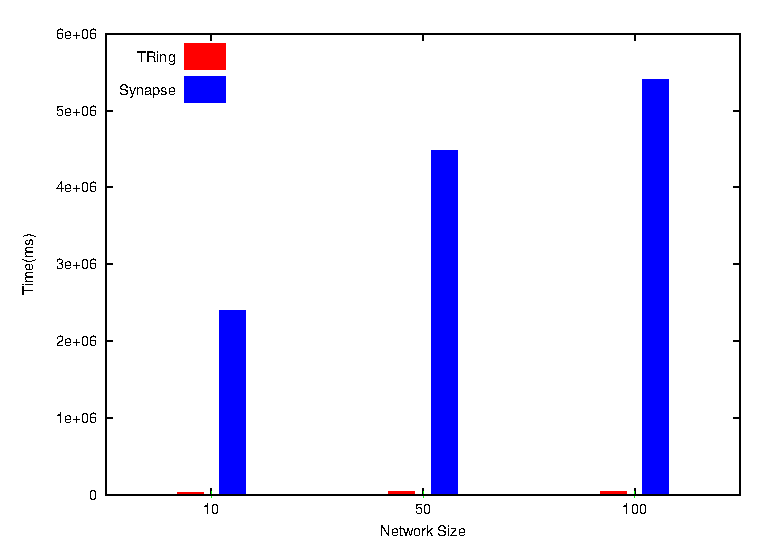
\includegraphics[width=14cm]{./images/compare_retrieve_rtt50.eps}
\begin{center}
  \begin{tabular}{|c||c|c|c|} \hline
  \backslashbox{}{} & NS=10 & NS=50 & NS=100  \\ \hline \hline
       T-Ring & 25730 ms & 46740 ms & 45068 ms  \\ \hline
       Synapse & 2392797  ms & 4477108 ms & 5406327 ms \\ \hline
  \end{tabular}
\end{center}
\caption{取得:RTT=50}
 \label{fig:compare_retrieve_rtt50}
 \end{minipage}
\end{figure}

\begin{figure}[htbp]
\begin{minipage}{1\textwidth}
    \centering
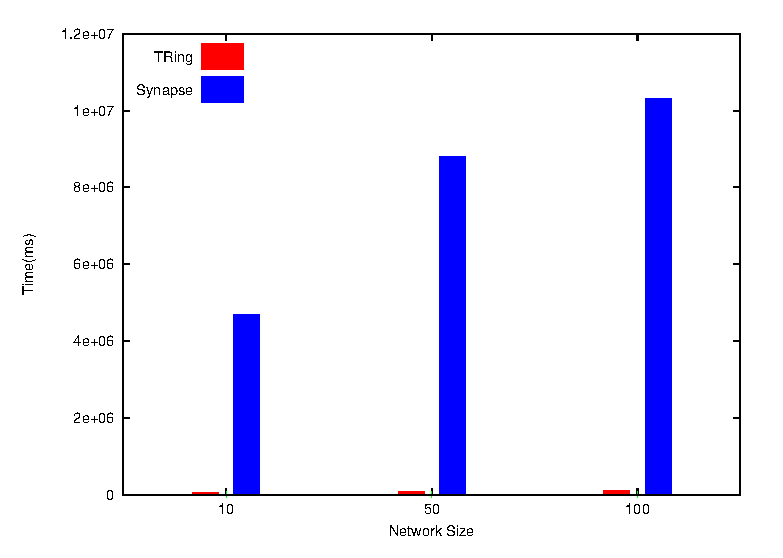
\includegraphics[width=14cm]{./images/compare_retrieve_rtt100.eps}
\begin{center}
  \begin{tabular}{|c||c|c|c|} \hline
  \backslashbox{}{} & NS=10 & NS=50 & NS=100  \\ \hline \hline
       T-Ring & 51478 ms & 90249 ms & 104476 ms  \\ \hline
       Synapse & 4691619  ms & 8816386 ms & 10322459 ms \\ \hline
  \end{tabular}
\end{center}
\caption{取得:RTT=100}
 \label{fig:compare_retrieve_rtt100}
 \end{minipage}
\end{figure}

\section{考察}
本節では,保存ピア探索の計算コスト,保存,取得それぞれの実験の結果に関しての考察を行う.
\subsection{保存ピア探索の計算コストにおける考察}
Synapseでは,保存される全てのデータに対して保存ピアの計算が行われる.つまり,ネットワークサイズ=N,データの数=D,ホップ数=Hとすると理論値では,
\begin{equation}
H=D\cdot\log{2}N \label{1}
\end{equation}
となる.(\ref{1})における$\log{2}N$は,Chordの平均探索ホップ数である.それに対してT-Ringでは,Synapseでの所与の変数に加え,chunkの時間=C,SPの時間=S,保存されるデータの時間間隔=IT,保存されるデータの総時間=ATと,時間的な変数を加えて考えると,理論値は,
\begin{equation}
D= \frac{AT}{IT} \label{2}
\end{equation}
\begin{equation}
H=\frac{AT}{C}- \frac{AT}{S} + \frac{AT}{S} \cdot\log{2}N \label{3}
\end{equation}
となり,(\ref{2})(\ref{3})から,ATを消去すると,
\begin{equation}
H=\frac{IT \cdot D\{S - C (1- \log{2}N ) \} }{C \cdot S} \label{4}
\end{equation}
(\ref{4})となる.
(\ref{1})(\ref{4})から,SynapseとT-Ringにおけるホップ数(それぞれSynapseH,T-RingH)の割合を計算すると,
\begin{equation}
\frac{SynapseH}{TRingH}=\frac{1}{IT} \cdot \frac{S \cdot C \cdot \log{2}N }{S + C(\log{2}N -1)}     \label{5}
\end{equation}
ここから,chunkとSPの関係性について考えると,
\begin{equation}
C \cdot S \cdot \log{2}N - S + C(\log{2}N - 1) = C \cdot \log{2} N \cdot (S+1) - ( S + C )
\end{equation}
と$C>S>0$,$N>0$から,SPの値が大きくなる場合,chunkの値がSPの値に近づく場合,(\ref{5})の値が大きくなる.また,同様にITの値が小さくなるほど,(\ref{5})の値が大きくなる.

ここから,実験結果を考察すると,実験結果は,理論値とほぼ相違ないことが分かる.よって,今回はchunk,SP,データの保存間隔を以上で述べた通りに行ったが,chunk=999,SP=1000,データの保存間隔=1にした場合,Synapseのホップ数に限りなく近づく.

この保存ピア探索の計算コストは,データの保存,取得に大きく関係する.次節からこの関係性について考察する.
\subsection{データ保存における考察}
前節において,保存ピア探索の計算コストについての考察を行ったが,SynapseとT-Ringのデータの保存にかかる時間の割合は,ネットワークレイテンシ(RTT)=RTTとすると,
\begin{equation}
\frac{SynapseH}{TRingH} \cdot RTT \cdot D \label{6}
\end{equation}
となる,SynapseとT-Ringを比較した際,RTTとDは同一の環境で実験をした場合,値の違いはないので,$\frac{SynapseH}{TRingH}$において,取得時間は決定する.ここから,実験結果を考察すると,T-Ringにおける取得時間が理論値以上であることが伺える.これは,センサデータの保存を行う前段階のセンサ情報の取得による影響であると考えられる.本システムでは,センサデータがセンサノードから保存ピアに送られた際,そのセンサデータの時間とそのセンサノードの設置時間から,対象のデータの保存先が次の保存ピアに移行するのか,移行する際,異なるマスターノードに移行するのかを計算する.この計算に時間を要する分,T-Ringが理論値と異なっていると考えられる.

\subsection{データの取得における考察}
データの取得においても,保存時と同様に考え,クエリの検索範囲の半径=Rとすると,SynapseとT-Ringのデータの保存にかかる時間の割合は,
\begin{equation}
\frac{SynapseH}{TRingH} \cdot RTT \cdot D \cdot  \pi r^{2}  \label{7}
\end{equation}
となる.保存時と比較すると,対象範囲内の全ての座標を計算するため,$\pi r^{2}$倍の差が発生することとなる.このことが,実験結果において,SynapseとT-Ringの時間の差が発生した論拠であると考えられる.

\section{まとめ}
本章では,まず,本研究に評価方針,実験環境を述べた.次に,実験環境内における実験への影響を調査するため,それぞれのリージョンからICMPにおける,Message Requestを送信し,リプライが返されるまでの時間(RTT)を計測した.その結果,RTTは0.400ms以内であり,十分に無視できることを述べた.次いで,保存ピア探索における計算コスト,データの保存に要する時間,データの取得に要する時間の観点から評価を行った.その結果から,考察を行い,理論値と実際の値に齟齬が存在することを明らかにし,その違いは,T-Ringにおいて,保存や取得の対象となるデータの時間情報の取得を行う際に要する時間により生じていることに言及した.